\section{The gap between human and LLM thinking, and how a BLLM closes it}\label{sec:gap}

The theorems so far price the checking of what a proposer proposes. They are silent on the proposer itself, and a sound system whose proposer never reaches the right idea is sound and useless. Chen, Zhao and Cohan have measured how far the ideas of language models are from those of human researchers \cite{CZC26}.\footnote{Z.~Chen, Y.~Zhao and A.~Cohan, \emph{Measuring the gap between human and LLM research ideas}, preprint (1 July 2026), arXiv:2607.01233 \cite{CZC26}. For each of 11{,}683 papers of ICLR, ICML and NeurIPS (2023 to 2026) and of Nature Communications (2023 to 2025) they reconstruct a small set of prior works that likely inspired its core idea, ask a language model for a new idea from the titles and summaries of those works, and classify the human idea and the generated ones on two axes of seven classes: the kind of research opportunity (puzzle or contradiction, explanation gap, scope mismatch, evidence gap, bridge opportunity, failure or risk gap, resource bottleneck) and the kind of method (synthesis or unification, relaxing or extending the scope, robustification, formal derivation, empirical mapping, artifact or system, optimisation or search). They conclude that the range of the generated ideas is narrower than, and systematically shifted from, the human one. The shares used here are those of their Figure~3, read from the vector paths of the figure to $0.1$ percentage points and checked against the counts of their Table~11 and the distances of their Table~1.} Other measurements of the same gap, between the language a model produces and the reasoning it is asked for \cite{LCL25} and between human and model reasoning on naturalistic detective problems \cite{LG26}, point the same way. This section turns the measurement into a law: it computes, from the measured profiles, how many proposals a model needs to reach the kind of idea a problem calls for, proves the least possible number, and shows that a selector which learns from the checks reaches that least number.

\subsection{The gap law}

Ideas fall into $K$ classes. A problem needs an idea of class $j$ with probability $\pi_{j}$, its \emph{need}, and a proposer draws the classes of its proposals independently from a profile $q$ until it draws the needed class. The expected number of proposals is
\begin{equation}\label{eq:searchcost}
C(\pi,q)=\sum_{j}\pi_{j}\,\EE[\text{draws until }j]=\sum_{j}\frac{\pi_{j}}{q_{j}} .
\end{equation}
Write $S=\sum_{j}\sqrt{\pi_{j}}$, $r_{j}=\sqrt{\pi_{j}}/S$ and $H_{1/2}(\pi)=2\log S$, the R\'enyi entropy of order one half \cite{Ren61}; $\chi^{2}(r\|q)=\sum_{j}(r_{j}-q_{j})^{2}/q_{j}$ is the chi-squared divergence.

\begin{mainthm}[Gap law]\label{thm:I}
For every need $\pi$ and every profile $q$ with $q_{j}>0$,
\begin{enumerate}[label=\textup{(\roman*)},leftmargin=2.2em,itemsep=1pt]
\item $C(\pi,q)\ge S^{2}=e^{H_{1/2}(\pi)}$, with equality exactly at $q=r$, square-root sampling;
\item $C(\pi,q)=e^{H_{1/2}(\pi)}\bigl(1+\chi^{2}(r\|q)\bigr)$;
\item for every $\lambda\in(0,1]$ the mixture $q_{\lambda}=(1-\lambda)q+\lambda r$ has $C(\pi,q_{\lambda})\le e^{H_{1/2}(\pi)}/\lambda$, whatever $q$ is;
\item a proposer that copies the need, $q=\pi$, pays $K\ge S^{2}$, with equality only for the uniform need.
\end{enumerate}
\end{mainthm}

\begin{proof}
(i) By the Cauchy--Schwarz inequality,
\[
S=\sum_{j}\sqrt{\frac{\pi_{j}}{q_{j}}}\,\sqrt{q_{j}}\le\Bigl(\sum_{j}\frac{\pi_{j}}{q_{j}}\Bigr)^{1/2}\Bigl(\sum_{j}q_{j}\Bigr)^{1/2}=C(\pi,q)^{1/2},
\]
with equality if and only if $\sqrt{\pi_{j}/q_{j}}$ is proportional to $\sqrt{q_{j}}$, that is $q_{j}\propto\sqrt{\pi_{j}}$. (ii) Since $\pi_{j}=S^{2}r_{j}^{2}$,
\[
\begin{aligned}C(\pi,q)&=S^{2}\sum_{j}\frac{r_{j}^{2}}{q_{j}}=S^{2}\Bigl(1+\sum_{j}\frac{r_{j}^{2}}{q_{j}}-2\sum_{j}r_{j}+\sum_{j}q_{j}\Bigr)\\&=S^{2}\bigl(1+\chi^{2}(r\|q)\bigr).\end{aligned}
\]
(iii) Coordinatewise $q_{\lambda,j}\ge\lambda r_{j}$, so $C(\pi,q_{\lambda})\le\sum_{j}\pi_{j}/(\lambda r_{j})=S\sum_{j}\sqrt{\pi_{j}}/\lambda=S^{2}/\lambda$. (iv) $C(\pi,\pi)=\sum_{j}1=K$, and $S^{2}\le K\sum_{j}\pi_{j}=K$ by the Cauchy--Schwarz inequality, with equality only when all $\pi_{j}$ are equal.
\end{proof}

Parts (i) to (iii) are proved in Lean (Appendix~\ref{app:checks}). Square-root sampling is the rule found by Press for the screening of rare cases \cite{Pre09}; here it answers a different question, and its meaning is plain. A proposer that follows the needs too closely wastes its proposals on the common classes, which are found quickly anyway, and a proposer that ignores them never reaches the rare ones; the optimum spends on each class in proportion to the square root of its need. Part (iv) says that even a proposer with perfect human taste, one that proposes as often as humans succeed, is not optimal: it pays $K$ against $S^{2}$. The gap of a proposer is the chi-squared divergence of its profile from square-root sampling, and part (iii) says that it closes at once, by a factor that does not depend on the proposer, as soon as a fixed fraction of the proposals is drawn from the right profile.

\subsection{The gap, measured}

We take as need the human profile: the class of idea a problem required is the class its authors used. Table~\ref{tab:gap} gives the cost \eqref{eq:searchcost} of each model of \cite{CZC26} on both axes, the cost of the half-and-half mixture with square-root sampling, and the least weight $\lambda$ on square-root sampling that brings the cost within $10\%$ of the optimum. On the axis of opportunities the optimum is $S^{2}=6.503$ proposals per problem and the human profile pays $7$; the models pay between $12.69$ (Gemini~3.1~Pro) and $27.81$ (GPT-OSS-120B), from $1.95$ to $4.28$ times the optimum. Nearly all of the gap comes from one class: the models propose ``bridge opportunities'', the transfer of a method from one field to another, in $47$ to $64\%$ of their ideas (Gemini~3.1~Pro $46.9\%$, GPT-OSS-120B $64.2\%$) against $12\%$ of the human ones, and evidence gaps and scope mismatches, $28\%$ of the human ideas, in $5$ to $11\%$ (Fig.~\ref{fig:gap}(a)). On the axis of methods the models pay from $1.51$ to $3.28$ times the optimum, with the excess in synthesis and unification.

\begin{table*}[t]
\caption{The gap, from the data of \cite{CZC26}, with the human profile as need. ``Cost'' is the expected number of proposals per problem \eqref{eq:searchcost}; ``ratio'' is the cost over the optimum $e^{H_{1/2}(\pi)}$, equal to $1+\chi^{2}(r\|q)$ by Theorem~\ref{thm:I}(ii); ``TVD'' is the total variation distance from the human profile; ``50/50'' is the cost of the mixture with weight $\frac12$ on square-root sampling, at most $2e^{H_{1/2}(\pi)}$ by Theorem~\ref{thm:I}(iii); ``steer'' is the least weight on square-root sampling that brings the cost within $10\%$ of the optimum, at most $1/1.1=0.909$ for every proposer.}
\label{tab:gap}
\centering
\footnotesize
\setlength{\tabcolsep}{4.5pt}
\begin{tabular}{@{}l rrrrr c rrrrr@{}}
\toprule
 & \multicolumn{5}{c}{research opportunity, optimum $6.503$} && \multicolumn{5}{c}{method, optimum $6.445$} \\
\cmidrule{2-6}\cmidrule{8-12}
Proposer & cost & ratio & TVD & 50/50 & steer && cost & ratio & TVD & 50/50 & steer \\
\midrule
Human profile & 7.00 & 1.08 & 0.000 & 6.62 & 0.00 && 7.00 & 1.09 & 0.000 & 6.57 & 0.00 \\
Claude Sonnet 4.6 & 14.14 & 2.17 & 0.352 & 7.73 & 0.64 && 9.74 & 1.51 & 0.211 & 7.04 & 0.48 \\
Gemini 3.1 Pro & 12.69 & 1.95 & 0.349 & 7.66 & 0.63 && 10.96 & 1.70 & 0.227 & 7.15 & 0.52 \\
GPT-OSS-20B & 23.70 & 3.64 & 0.457 & 8.48 & 0.72 && 21.15 & 3.28 & 0.378 & 7.89 & 0.66 \\
GPT-OSS-120B & 27.81 & 4.28 & 0.522 & 8.74 & 0.74 && 20.94 & 3.25 & 0.390 & 7.90 & 0.66 \\
GPT-5.4 mini & 27.69 & 4.26 & 0.511 & 8.61 & 0.73 && 11.84 & 1.84 & 0.339 & 7.45 & 0.60 \\
Qwen3-8B & 23.38 & 3.59 & 0.383 & 8.17 & 0.69 && 20.99 & 3.26 & 0.368 & 8.00 & 0.68 \\
Qwen3-32B & 20.67 & 3.18 & 0.418 & 8.26 & 0.70 && 19.78 & 3.07 & 0.364 & 7.93 & 0.67 \\
DeepSeek V4 Flash & 16.89 & 2.60 & 0.401 & 8.03 & 0.68 && 12.93 & 2.01 & 0.246 & 7.21 & 0.54 \\
DeepSeek V4 Pro & 24.35 & 3.74 & 0.437 & 8.30 & 0.70 && 12.11 & 1.88 & 0.258 & 7.38 & 0.58 \\
Square-root sampling & 6.50 & 1.00 & 0.099 & 6.50 & 0.00 && 6.44 & 1.00 & 0.119 & 6.44 & 0.00 \\
\bottomrule
\end{tabular}
\end{table*}

Two facts in the table are worth stating separately. The ranking by cost is not the ranking by distance: on the axis of opportunities Qwen3-8B is closer to the human profile than Qwen3-32B and DeepSeek~V4~Flash and costs $13\%$ and $38\%$ more, and on the axis of methods GPT-5.4 mini is farther from it than DeepSeek~V4~Pro and costs less. The cost weighs a class by its need over its share, so a class that a model almost never proposes costs it far more than the distance records. And the mixtures of the table close most of the gap at a moderate price: half the proposals from square-root sampling bring every model within $1.35$ times the optimum on opportunities and $1.25$ times on methods, and a weight between $0.48$ and $0.74$ brings it within $10\%$.

\begin{figure*}[t]
\centering
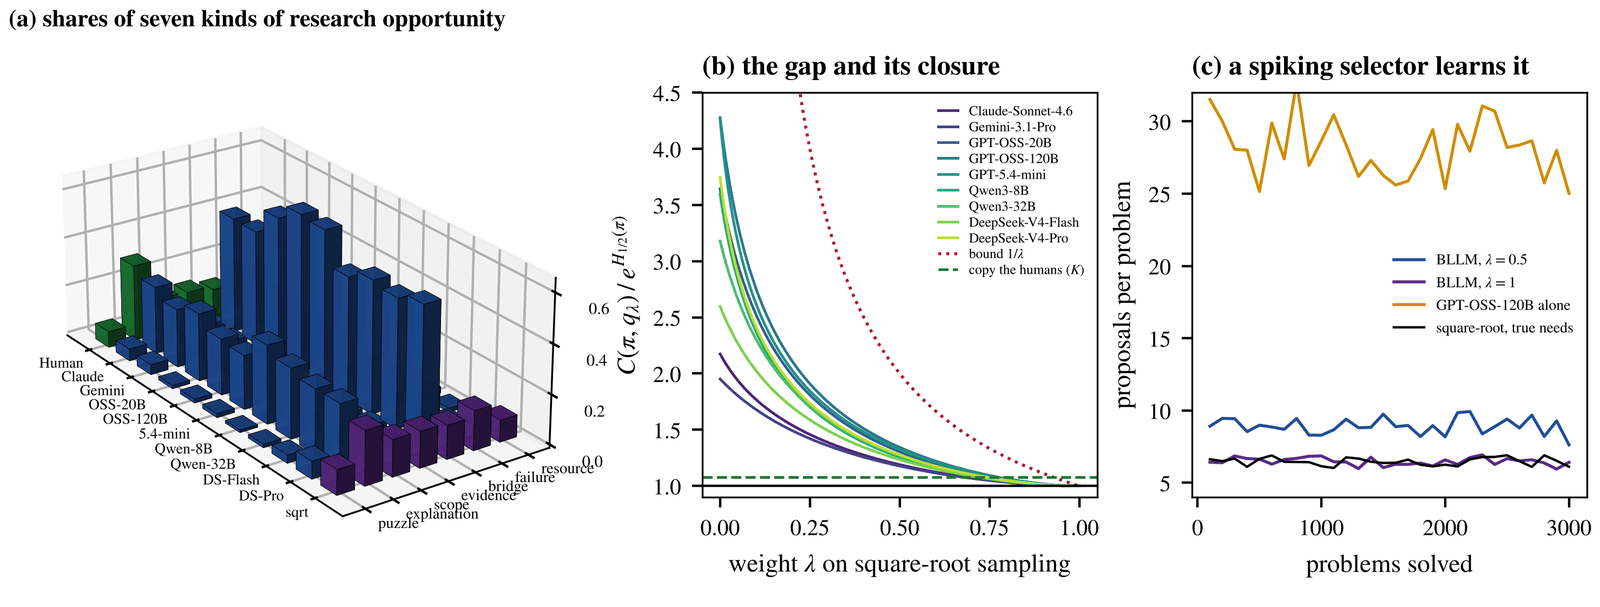
\includegraphics[width=0.98\textwidth]{figures/fig_gap}
\caption{The gap between human and LLM research ideas and its closure. (a) The shares of the seven kinds of research opportunity in the human papers and in the ideas of nine language models \cite{CZC26}, and square-root sampling of the human profile (``sqrt''); the models concentrate on bridge opportunities. (b) The cost of the mixture $q_{\lambda}$ of each model with square-root sampling, divided by the optimum $e^{H_{1/2}(\pi)}$, against the weight $\lambda$: every curve lies below the bound $1/\lambda$ of Theorem~\ref{thm:I}(iii), dotted, and falls below the cost of the human profile, dashed, at a weight between $0.68$ and $0.78$. (c) A stream of $3000$ problems with the opportunity profile of GPT-OSS-120B, mean proposals per problem over windows of $100$ problems and six seeds: the model alone pays $28.1$ against the $27.81$ of the law; a BLLM that draws half of its proposals from the spiking selector of Section~\ref{ssec:selector}, which learns only from the problems its checks close, pays $8.9$, the value $8.74$ of the law; with all proposals from the selector it pays $6.45$, the optimum $6.50$ of square-root sampling with the true needs.}
\label{fig:gap}
\end{figure*}

\subsection{Learning the need from the checks}

Square-root sampling needs $\pi$, and $\pi$ is not given. A BLLM learns it from its own record: every result its checks keep closes a problem with an idea of a known class, so after $n$ closed problems it has counts $c_{j}$ with $\sum_{j}c_{j}=n$, and it samples from the square root of the estimate $\hat\pi_{j}=(c_{j}+\alpha)/(n+K\alpha)$, with a prior count $\alpha>0$. The next proposition says how fast this closes the gap.

\begin{proposition}[Learning rate]\label{prop:learnrate}
Let the counts be multinomial with parameters $n$ and $\pi$, all $\pi_{j}>0$, and let $\hat r$ be square-root sampling of $\hat\pi$. Then
\begin{equation}\label{eq:learnrate}
\begin{gathered}\frac{\EE\,C(\pi,\hat r)}{e^{H_{1/2}(\pi)}}=1+\frac{\beta(\pi)}{4n}+o\Bigl(\frac1n\Bigr),\\ \beta(\pi)=\frac1S\sum_{j}\frac{1}{\sqrt{\pi_{j}}}-\frac{K}{S^{2}}\ \ge\ \frac{K(K-1)}{S^{2}} .\end{gathered}
\end{equation}
\end{proposition}

\begin{proof}
By Theorem~\ref{thm:I}(ii) the ratio is $1+\EE\,\chi^{2}(r\|\hat r)$. Write $\hat\pi=\pi+d$. The map $x\mapsto\chi^{2}(r\|\rho(x))$, with $\rho_{j}(x)=\sqrt{x_{j}}/\sum_{k}\sqrt{x_{k}}$, is smooth near $\pi$, vanishes at $\pi$ with its gradient, and its second-order part is computed from $\rho_{j}(\pi+d)-r_{j}=(u_{j}-r_{j}U)/S+O(|d|^{2})$, where $u_{j}=d_{j}/(2\sqrt{\pi_{j}})$ and $U=\sum_{j}u_{j}$:
\[
\begin{aligned}\chi^{2}(r\|\rho(\pi+d))&=\frac1S\sum_{j}\frac{(u_{j}-r_{j}U)^{2}}{\sqrt{\pi_{j}}}+O(|d|^{3})\\&=\frac1S\Bigl(\sum_{j}\frac{u_{j}^{2}}{\sqrt{\pi_{j}}}-\frac{U^{2}}{S}\Bigr)+O(|d|^{3}),\end{aligned}
\]
using $r_{j}/\sqrt{\pi_{j}}=1/S$ and $\sum_{j}r_{j}^{2}/\sqrt{\pi_{j}}=1/S$. The prior shifts the mean of $d$ by $O(1/n)$, and the covariance of $d$ is $(\mathrm{diag}(\pi)-\pi\pi^{\top})/n+O(n^{-2})$; so $\EE u_{j}^{2}=(1-\pi_{j})/(4n)+O(n^{-2})$ and $\EE U^{2}=\frac1{4n}\bigl(\sum_{j}(1-\pi_{j})-\sum_{j\ne k}\sqrt{\pi_{j}\pi_{k}}\bigr)+O(n^{-2})=\frac{K-S^{2}}{4n}+O(n^{-2})$. Substituting,
\[
\EE\,\chi^{2}=\frac1{4nS}\Bigl(\sum_{j}\frac{1-\pi_{j}}{\sqrt{\pi_{j}}}-\frac{K-S^{2}}{S}\Bigr)+o\Bigl(\frac1n\Bigr)=\frac{\beta(\pi)}{4n}+o\Bigl(\frac1n\Bigr),
\]
since $\sum_{j}(1-\pi_{j})/\sqrt{\pi_{j}}=\sum_{j}\pi_{j}^{-1/2}-S$. The remainder is $o(1/n)$: on the event $|d|\le\delta$ it is bounded by a constant times $\EE|d|^{3}=O(n^{-3/2})$, and off it $\chi^{2}(r\|\hat r)$ is at most a polynomial in $n$, because $\hat\pi_{j}\ge\alpha/(n+K\alpha)$, while the event has probability $e^{-cn}$ by Hoeffding's inequality \cite{Hoe63}. Finally $\sum_{j}\pi_{j}^{-1/2}\ge K^{2}/S$ by the Cauchy--Schwarz inequality, which gives the lower bound on $\beta$.
\end{proof}

For the human profile of opportunities $\beta=7.06$, so a BLLM that has closed $100$ problems pays $1.018$ times the optimum, and after $1000$ problems $1.0018$ times; simulation gives $1.019$ and $1.0018$, and at $n=20$, where the expansion is not yet accurate, $1.083$. The correction is of order $K^{2}/n$ and does not depend on the proposer at all: the gap of a language model is a fixed multiple, the gap of a learning selector disappears like $1/n$.

\subsection{A spiking selector}\label{ssec:selector}

The selector that the BLLM package uses is a circuit of spiking neurons, chosen because it computes square-root sampling exactly with the elements and the learning rule that nervous systems use for the selection of actions \cite{RPG99,SDM97,FG16} and that neuromorphic hardware implements \cite{Mea90,Maa97,DSL18}. There is one leaky integrate-and-fire neuron for each class, or for each agent; the membrane potential $u_{k}$ of neuron $k$ relaxes with time constant $\tau$ to its synaptic drive $w_{k}$, and the neuron fires in continuous time with the escape rate $\rho_{0}e^{(u_{k}-\vartheta)/\delta}$ \cite{GKN14}. The first neuron to fire chooses. When a check keeps a result produced by class $k$, a reward, the third factor of a three-factor rule \cite{FG16}, potentiates that synapse,
\begin{equation}\label{eq:spikereward}
w_{k}\leftarrow w_{k}+\frac\delta2\log\frac{c_{k}+1+\alpha}{c_{k}+\alpha},\qquad c_{k}\leftarrow c_{k}+1,
\end{equation}
and synaptic scaling \cite{TLD98} then shifts all weights by a common amount that keeps the total rate equal to $\rho_{0}$.

\begin{proposition}[The selector samples the square root of what it has learned]\label{prop:spiking}
Once the membranes have relaxed, the neuron that fires first is $k$ with probability $e^{w_{k}/\delta}/\sum_{l}e^{w_{l}/\delta}$, and after the rewards \eqref{eq:spikereward} this probability is $\sqrt{c_{k}+\alpha}/\sum_{l}\sqrt{c_{l}+\alpha}$, square-root sampling of the estimated need $\hat\pi$.
\end{proposition}

\begin{proof}
With relaxed membranes, $u_{k}=w_{k}$ and the neurons fire as independent Poisson processes of rates $\lambda_{k}=\rho_{0}e^{(w_{k}-\vartheta)/\delta}$. The first spike of neuron $k$ is exponential with rate $\lambda_{k}$, and the least of independent exponential times is the $k$-th with probability $\lambda_{k}/\sum_{l}\lambda_{l}$. The increments \eqref{eq:spikereward} telescope, so after $c_{k}$ rewards $w_{k}=w_{k}(0)+\frac\delta2\log\frac{c_{k}+\alpha}{\alpha}$, and the scaling adds the same constant to every $w_{l}$, which cancels in the ratio. With equal initial weights, $e^{w_{k}/\delta}$ is proportional to $\sqrt{c_{k}+\alpha}$.
\end{proof}

In the package the membranes are integrated with a step $\mathrm{d}t$ and the race opens after five time constants, so the probabilities hold up to terms of order $\rho_{0}\,\mathrm{d}t$ and $e^{-5}$; over $40{,}000$ races they agree with $\sqrt{c_{k}+\alpha}/\sum_{l}\sqrt{c_{l}+\alpha}$ to within $0.007$. Combined with Proposition~\ref{prop:learnrate}, the circuit closes the gap at the rate $\beta/(4n)$, and it does so with nothing a nervous system lacks: a race to threshold, a reward that potentiates the winner, and a homeostatic scaling of the total rate. Figure~\ref{fig:gap}(c) shows it on the profile of GPT-OSS-120B. The selector never decides a result; it only chooses which class, or which agent, proposes next, and every proposal meets the checks, so the soundness of Theorems~\ref{thm:A} to~\ref{thm:H} is untouched and the gap law is a statement about cost alone.

\subsection{What the gap law says, and what it does not}

The law is exact for its model: independent proposals, a need that is a distribution over classes, and a proposer that keeps drawing until the class is right. Reaching the right class is necessary for reaching the right idea, not sufficient, and within a class a proposer may still fail; that part is priced by the checks, and the two costs multiply. The need is taken from the human papers, which is the only meaning the measurement of \cite{CZC26} gives to the right class; if the human profile is itself biased, square-root sampling of a better need is better still, and the law applies unchanged. What the law gives is a closed form for the cost of the gap that was measured, the proof that this cost is a chi-squared divergence from square-root sampling, a universal bound for its closure, and a circuit that reaches the optimum by learning from its checks at the rate $\beta/(4n)$. It does not make a language model think like a person. It makes a system that contains a language model search for ideas, at the level of the classes measured, with fewer proposals than either the model or a proposer with human taste.
